\documentclass[letterpaper,twocolumn,amsmath,amssymb,prb]{revtex4-1}
\usepackage{graphicx}% Include figure files
\usepackage{dcolumn}% Align table columns on decimal point
\usepackage{bm}% bold math
\usepackage{color}

%%%%%%%%%%%%%%%%%%%%%%%%%%%%%%%%%%%%%%%%%%%%%%%%%%%%%%%%%%%%
%% Definitions
\def\re{\text{Re}}
\def\im{\text{Im}}
\def\ket#1{\vert #1 \rangle}
\def\cU{{\cal{U}}}
\def\cD{{\cal{D}}}
\def\re{\text{Re}}
\def\im{\text{Im}}
\newcommand{\red}[1]{{\bf \color{red} #1}}
\newcommand{\blue}[1]{{\bf \color{blue} #1}}
\newcommand{\green}[1]{{\bf \color{green} #1}}
\newcommand{\rr}{\textbf{r}}
\newcommand{\xx}{\textbf{x}}
\newcommand{\refnote}{\red{[ref]}}

\newcommand{\fixme}[1]{\red{[#1]}}

% needsworklater is used to annotate bits that need work, but that we
% can postpone for a while.
\newcommand{\needsworklater}[1]{\emph{[#1]}}
% needsworknow is intended to prioritize stuff that needs fixing.
\newcommand{\needsworknow}[1]{\textcolor{red}{[\emph{#1}]}}

%%%%%%%%%%%%%%%%%%%%%%%%%%%%%%%%%%%%%%%%%%%%%%%%%%%%%%%%%%%%

\begin{document}
\title{A Classical Density-Functional Theory for Describing Water Interfaces}

\author{Jessica Hughes}
\affiliation{Department of Physics, Oregon State University, Corvallis, OR 97331}
\author{Eric Krebs}
\affiliation{Department of Physics, Oregon State University, Corvallis, OR 97331}
\author{David Roundy}
\affiliation{Department of Physics, Oregon State University, Corvallis, OR 97331}

%%%%%%%%%%%%%%%%%%%%%%%%%%%%%%%%%%%%%%%%%%%%%%%%%%%%%%%%%%%%
\begin{abstract}
{We develop a classical density functional theory for water by combining the
fundamental-measure theory functional--which describes hard sphere fluids--with
attractive interactions based on the Statistical Associating Fluid Theory
(SAFT-VR). Using this approximation with an additional length scale parameter, we are able to calculate the vapor pressure, saturated liquid density, surface tension, and enthalpy of water, as well as the number of hydrogen bonds and density oscillations formed near hydrophobic rods and spheres immersed in water. 
\needsworknow{For two rods being pulled apart, a transition occurs 
from a vapor state to a liquid state in the area between
the rods at approximately $(\pi-2)$ multipled by the radius. Even 
for nanoscale rods (radius 0.5~-~1.0~nm), we find that in the
vapor state, the force can be approximated
classically and is equal to 144~mN/m, or twice the bulk surface tension.
(Edit this and add spheres stuff)}
This functional is computationally efficient and provides a foundation for 
future work describing complex interactions in aqueous solution on an
atomic level.}
\tableofcontents
\end{abstract}
\maketitle

{\begin{itemize}
\color{blue}
\item Put finished things up here
\item[JRH] Rewrite abstract (copying from project)
\item[JRH] Cut the test-particle section
\item[JRH] Rewrite and join introductions
\item[JRH] Decide what to do with slit (cut)
\item[JRH] Combine and edit Other Thermo and Empirical Parameters sections
\color{red}
\item[JRH] Work on abstract
\item[DJR] Read and edit changes to abstract and introduction
\item[DJR] Look through theory section for stuff to cut
\item[DJR,JRH] Finalize figures in beginning
\item[JRH] Better/expanded description of ``macroscopic surface tension'' model in 2 rods section?
\item[JRH] Recalculate and clean up 2 rods figures and data - new code?
\item[DJR] Write text (or clean up existing) for hard sphere solutes
\item[EJK] Add 4-rods figures
\item[EJK] Add 4-rods text
\item[JRH,DJR] Rewrite conclusion
\end{itemize}
}


%%%%%%%%%%%%%%%%%%%%%%%%%%%%%%%%%%%%%%%%%%%%%%%%%%%%%%%%%%%%
\section{Introduction}

\subsection{Water---the universal solvent}

A large fraction of interesting chemistry---including all of molecular
biology---takes place in aqueous solution.  However, while quantum
chemistry now enables us to calculate the ground state energies of
large molecules in vacuum, prediction of the free energy of even the
smallest molecules in the presence of a solvent poses a continuing
challenge due to the complex structure of a liquid and the
computational cost of \emph{ab initio} molecular
dynamics~\cite{car1985, grossman2004}.  The current state-of-the art
in \emph{ab initio} molecular dynamics is limited to around 64 water
molecules per unit cell, which places the minimum solute concentration
at 0.84 molar and allows contact between the second solvation shell of
neighboring solutes~\cite{izvekov2005, choe2007}.  On top of this,
\emph{ab initio} approaches using classical molecular dynamics have
\textcolor{red}{vague problems}\cite{weber2010ab-initio-water}.  A
more efficient approach is needed in order to study nanoscale and
hydrophobic solutes.

Water stands out among liquids for its extraordinary properties.  Water is
the only natural substance that is found in solid, liquid and gaseous
states at temperatures and pressures normally found on Earth.  Water has a
density maximum at 4$^\circ$C, and expands upon freezing.  The heat
capacity of water is the highest of any liquid, and its latent heat of
fusion and vaporization are also the highest.  Water's thermal conductivity
and surface tensions are the highest of any non-metallic liquid.  Water has
an unusually high dielectric constant.
Much of the unusual behavior of water is explained by the ability of each
water molecule to form \emph{four} strong, directional hydrogen bonds---two
acceptors and two donors.  This directional bonding dictates the open
structure of ice, leading to thermal expansion upon freezing.

Due to its large dielectric constant, small molecular size and strong
hydrogen-bonding network, water as ``the universal solvent'' is as
interesting as its anomalous thermodynamic properties.

\subsection{Classical density-functional theory}

%\begin{figure}
%\includegraphics[width=6cm, angle=270]{figs/correlation}
%\caption{ Experimental atom-atom radial distribution functions for water at
%room temperature and pressure from reference~\cite{Soper2000}.\needsworknow{Either 
%mention this figure in the text or delete it.}  }
%\label{correlation}
%\end{figure}

Numerous approaches have been developed to approximate the effect of water
as a solvent in atomistic calculations.  Each of these approaches gives
adequate description of some aspect of interactions with water, but none of
them is adequate for describing \emph{all} these interactions with an
accuracy close to that attained by \emph{ab initio} calculations.  The
theory of Lum, Chandler and Weeks (LCW)~\cite{lum1999hydrophobicity}, for 
instance, can
accurately describe the free energy cost of creating a cavity by placing a
solute in water, but does not lend itself to extensions treating the strong
interaction of water with hydrophilic solutes.  Treatment of water as a
continuum dielectric with a cavity surrounding each solute can give
accurate predictions of the energy of solvation of ions~\cite{latimer1939,
rashin1985, zhan1998, hsu1999, hildebrandt2004, hildebrandt2007}, but
provides no information about the size of this cavity.  In a physically
correct approach, the size of the cavity will naturally arise from a
balance between the free energy required to create the cavity, the
attraction between the water and the solute, and the steric repulsion which
opens up the cavity in the first place.

A very promising approach for an efficient continuum description of water
is that of classical density-functional theory (DFT), which is an approach
for evaluating the free energy and thermally averaged density of fluids in
an arbitrary external potential~\cite{ebner1976density}. The Hohenberg-Kohn
theorem\cite{hohenberg1964inhomogeneous} allows us to write the ground state
energy in terms of a universal functional of the electron density and a separate
term including the external potential. Mermin\cite{mermin1965thermal} gives a
theorem extending that of Hohenberg and Kohn to nonzero temperatures:
\begin{equation}
  A(T) = \underset{n(r)}{min}\left\{ F[n(r),T] + \int V_{ext}(r) n(r)
d^3r\right\}.
\end{equation}
This is the basis for classical DFT, where the relevant density is not the
electron density, but the density of molecules. Classical DFT is a
natural framework for creating a more flexible theory of hydrophobicity
that can describe interaction of water with arbitrary external
potentials---including potentials describing a \emph{strong} interaction
with a solute.
 
A number of exact properties are easily achieved in the density-functional
framework, such as the relationship between the pressure on a hard wall and
the contact density---which ensures a correct solvation free energy for
small hard solutes.  Much of the research on classical density-functional
theory has focused on the hard-sphere fluid~\cite{curtin1985,
rosenfeld1989, rosenfeld1993, rosenfeld1997, tarazona1997, tarazona2000}.
This has led to a large number of very sophisticated functionals, such as
the fundamental-measure theory (FMT) functional~\cite{rosenfeld1989,
rosenfeld1993, rosenfeld1997, tarazona1997, tarazona2000}.  This functional
\needsworknow{has many nice properties}.

Several classical density functionals have already been developed for
water~\cite{ding1987, Yang1992, Jaqaman2004}, capturing some of the
qualitative behavior of water.  However, many of these are less
sophisticated than those describing the hard-sphere fluid, and a
quantitatively accurate functional describing water---which reproduces both
the macroscopic surface tension and its decrease as curvature
increases---has not yet been published.  For instance, Jaqaman \emph{et al}
developed a classical density-functional for water including orientational
effects, but their functional resulted in a surface tension twice the
experimental value, with the result that it can really only be used to make
very qualitative predictions~\cite{Jaqaman2004}.

\needsworknow{Add discussion and citations for more recent papers}

One of the most interesting functionals for water is that of Ding \emph{et
al}, which was developed in order to explain the freezing of
water~\cite{ding1987}.  This functional uses the approach of Chandler
\emph{et al}, which uses separate atomic densities for the constituent
atoms of a molecular fluid~\cite{chandler1986a, chandler1986b}.  Although
this is a compelling approach, the actual functional developed cannot
describe the vapor state or liquid-vapor interface, both of which are
crucial to correct predictions of hydrophobic behavior at large length
scales.  In addition, the functional of Ding \emph{et al} also fails to
rigorously enforce intramolecular correlations, which casts doubt on its
suitability for describing interactions with ionic solutes.

\needsworknow{Add smooth transition from others' work to ours}

We use classical DFT to construct a new functional that will predict
the density of water molecules in a classical system.  The model we use
starts with a treatment of each individual water molecule as a purely
classical hard sphere and adds association terms based on Statistical 
Associating Fluid Theory (SAFT). Water, unlike simple
fluids which are mainly defined by van der Waals forces and weak electrostatic
interations, requires direct treatment of association effects. The strong 
hydrogen bonds and polar
interactions in water are ideal for describing with SAFT, which was designed for
use with such fluids. It is based on Wertheim's first-order
thermodynamic perturbation theory (TPT1)
\cite{wertheim1984fluidsI,wertheim1984fluidsII,wertheim1986fluidsIII,
wertheim1986fluidsIV} which provides a useful way to account for strong
associative interations between molecules. SAFT can account for the association energies
as well as any effects due to clusters or chains forming
in the liquid\cite{muller2001molecular}. \needsworknow{Expand or move this 
introduction to SAFT?}

\section{Theory and Methods}
We introduce a new classical density functional for water that
predicts the vapor pressure, vapor density, liquid density, bulk
surface tension, and enthalpy, as well as allows for liquid-vapor
coexistence.  The Helmholtz free energy functional is based on SAFT,
and is composed of the usual terms:
\begin{equation}
  F[n] = F_\textit{id}[n] + F_\textit{hs}[n]  +
F_\textit{disp}[n]+ F_\textit{assoc}[n],
\end{equation}
where $F_\textit{id}$ is the ideal gas free energy, $F_\textit{hs}$ is
the hard-sphere free energy, $F_\textit{disp}$ is the dispersion energy,
and $F_\textit{assoc}$ is the free energy of association.  In
addition, a chemical potential term is used, so we actually work in
the grand canonical ensemble.  In the following sections, we will
introduce the terms of this functional.

\subsection{Ideal gas functional}
The first term is the ideal gas free energy functional, which
incorporates effects of kinetic energy.  The ideal gas functional is
given by
\begin{equation}\label{idealgas}
  F_{id}[n] = k_B T \int n(\xx)\left( \ln{\frac{n(\xx)}{n_Q}} - 1\right) d\xx
\end{equation}
where n(\xx) is the density of water molecules and $n_Q$ is the
quantum concentration
\begin{equation}\label{quantumconcentration}
 n_Q =\left(\frac{mk_BT}{2\pi\hbar^2}\right)^{3/2}.
\end{equation}
The ideal gas free energy functional satisfies the contact density
theorem, which states that the contact density at a hard surface $n_c$
is proportional to the pressure on that surface. This
also leads to the property that the free energy of solvation of
a hard solute is proportional to its volume in the limit of small
solutes: 
\begin{equation}\label{contactvaluethm}
  F = n_c k_BT V\:.
\end{equation}
These properties are retained by the total functional,
provided the remaining terms are \emph{purely nonlocal}.  A common
failing of SAFT-based functionals (see, for instance
references\cite{felipe2001examination, gloor2002saft,
  gloor2004accurate, clark2006developing, gloor2007prediction,
  kahl2008modified, gross2009density}) is to treat other terms in the
functional locally, resulting in a functional that is suitable only
for studying the liquid-vapor interface.


\subsection{Hard-sphere repulsion}

We treat the repulsive interactions using the White Bear version of
the Fundamental-Measure Theory~(FMT) functional for the hard-sphere
fluid~\cite{roth2002whitebear}.  In the homogeneous limit, the White
Bear functional reduces to the Mansoori-Carnahan-Starling-Leland
equation of state.  FMT functionals are expressed as the integral of
the \emph{fundamental measures} of a fluid, which provide local
measures of quantities such as the filling fraction, density of
spheres touching a given point and mean curvature.  The excess free
energy is written as:
\begin{equation}
F_{hs}[n] = k_B T \int (\Phi_1(\xx) + \Phi_2(\xx) + \Phi_3(\xx)) d\xx \; ,
\end{equation}
with integrands
\begin{align}
\Phi_1 &= -n_0 \ln\left( 1 - n_3\right)\\
\Phi_2 &= \frac{n_1 n_2 - \mathbf{n}_{V1} \cdot\mathbf{n}_{V2}}{1-n_3} \\
\Phi_3 &= (n_2^3 - 3n_2 \mathbf{n}_{V2} \cdot \mathbf{n}_{V2})
  \frac{
    n_3 + (1-n_3)^2\ln(1-n_3)
  }{
    36\pi n_3^2\left( 1 - n_3 \right)^2
  } ,
\end{align}
where the fundamental measure densities are given by:
\begin{align}
  n_3(\xx) &= \int n(\xx') \Theta(\left|\xx - \xx'\right| - R) d\xx' \\
  n_2(\xx) &= \int n(\xx') \delta(\left|\xx - \xx'\right| - R) d\xx'
  \\
  \mathbf{n}_{V2} &= \mathbf{\nabla} n_3 \\
  n_1 &= \frac{n_2}{4\pi R}\\
  \mathbf{n}_{V1} &= \frac{\mathbf{n}_{V2}}{4\pi R}\\
  n_0 &= \frac{n_2}{4\pi R^2}.
\end{align}
The density $n_3$ is the filling fraction and $n_2$ describes the number
of spheres touching a given point. For our water functional, we use the 
hard-sphere radius of
3.03420~\AA, which was found to be optimal by Clark
\emph{et al}.\cite{clark2006developing}

\newcommand\etadisp{\ensuremath{\eta_\textit{d}}}
\newcommand\epsilondisp{\ensuremath{\epsilon_\textit{d}}}
\newcommand\epsilonassoc{\ensuremath{\epsilon_\textit{a}}}
\newcommand\kappaassoc{\ensuremath{\kappa_\textit{a}}}
\newcommand\lambdadisp{\ensuremath{\lambda_\textit{d}}}
\newcommand\lscale{\ensuremath{s_d}}
\subsection{Dispersion free energy}
The first term in the attractive energy is the dispersion term.  This
will include van der Waals attraction and any orientation-independent
interactions. We use a dispersion term based on the SAFT-VR
approach\cite{gil-villegas-1997-SAFT-VR}, which has two free
parameters, an interaction energy $\epsilondisp$ and a
length scale $\lambdadisp R$.

The dispersion free energy has the form~\cite{gil-villegas-1997-SAFT-VR}
\begin{align}
  F_\text{disp}[n] &= \int \left(a_1(\xx) + \beta a_2(\xx)\right)n(\xx)d\xx
\end{align}
where $a_1$ and $a_2$ are the first two terms in a high-temperature
perturbation expansion and $\beta=1/k_BT$.  The first term $a_1$ is 
the mean-field dispersion
interaction, which reduces in the homogeneous limit to
\begin{align}\label{eq:A1-simple}
  a_1 &= \frac12 n_b \int \varphi(\left|\xx\right|)
  g_{HS}(\left|\xx\right|) d\xx
\end{align}
where $n_b$ is the bulk density and $g_{HS}$ is the homogeneous
hard-sphere fluid correlation function.
The second dispersion term in the free energy $a_2$ describes the
effect of fluctuations resulting from the compression of the fluid due
to the dispersion interaction itself, and is commonly approximated
using the local compressibility approximation (LCA). In the LCA,
we assume the energy fluctuation is directly related to the
compressibility of a hard-sphere reference fluid\cite{barker1976liquid}.

We use a free square-well function for the dispersion $\varphi$, which
is the choice used by Clark \emph{et al}~\cite{clark2006developing},
and allows a reasonable fit to the equation of state.  Thus our model
interaction has the form:
\begin{equation}
  \varphi(r) = \Theta(r-2 \lambdadisp R)
\end{equation}
where $\Theta$ is the Heaviside step function.

The form of $a_1$ is given in
reference~\cite{gil-villegas-1997-SAFT-VR}, but is expressed in terms
of the filling fraction.  In order to apply this form to an
inhomogeneous density distribution, we construct an effective local
filling fraction for dispersion $\etadisp$, given by
\begin{align}
%    ((4/3.0*M_PI)*Pow(3)(R)*GaussianConvolve(2*lambdainput*lscale*radius,
%                                             2*lambdaE*length_scalingE*Rexpr)
%  \etadisp(\xx) &= \color{red}
%  \int \frac{\Theta(2\lambdadisp\lscale R - \left|\xx-\xx'\right|)}{
%             \left(2\lambdadisp\lscale\right)^3} n(\xx') d\xx'.
  \\
  \etadisp(\xx) &= \frac{1}{6\sqrt{\pi} \lambdadisp^3\lscale^3}
  \int n(\xx')\exp\left({-\frac{|\xx-\xx'|^2}{2(2 \lambdadisp
      \lscale R)^2}}\right)d\xx'
\end{align}
This effective filling fraction is used throughout the dispersion
calculations, and represents a filling fraction averaged over the
effective range of the dispersive interaction.  This functional
introduces an additional empirical parameter $\lscale$ which adjusts
the length scale over which the dispersion interaction is correlated.

The first term in the dispersion functional $a_1$ when written using
the above filling fraction for dispersion has the form
\begin{align}
  a_1 &= 
   -4(\lambdadisp^3 - 1)\epsilondisp \etadisp(\xx)
    g^{HS}_\sigma(\eta_\textit{eff}(\xx)) \\
  g_\sigma^{HS}(\eta) &= \frac{1 - \frac12 \eta}{(1 - \eta)^3} \label{eq:ghs}
  \\
  g_\sigma^{HS}(\eta) &= \frac{1}{1-\eta}
  +\frac32\frac{1}{(1-\eta)^2}
  + \frac12\frac{\eta^2}{(1-\eta)^3}
  \\
  \eta_\textit{eff}(\xx) &= \sum_{ij=0}^3 C_{ij}  \etadisp^i(\xx)
  \lambdadisp^j
\end{align}
where $g_\sigma^{HS}$
is the Carnahan-Starling value for the hard-sphere fluid correlation
function evaluated at contact.  \textcolor{red}{Jess, could you verify
that the two formulas for gHS above are equivalent? Thanks!}
The $C_{ij}$ values
 are numerical constants taken from
reference\cite{gil-villegas-1997-SAFT-VR}, which come from a numerical
fit to the integral in Equation~\ref{eq:A1-simple} over a range of
values for filling fraction and $\lambdadisp$.

The second term, $a_2$, which describes the contribution to the free
energy associated with fluctuations is given by
\begin{align}
  a_2 &= \frac12 \epsilondisp
              K_{HS}(\etadisp(\xx)) \etadisp(\xx)
              \frac{\partial a_1}{\partial \etadisp(\xx)}
\end{align}
where $K_{HS}$ is the Percus-Yevick hard-sphere compressibility, given
by
\begin{align}
  K_{HS} &=
    \frac{(1 - \etadisp)^4}{1 + 4(\etadisp + \etadisp^2)}.
\end{align}

\subsection{Association free energy}
The final attractive energy term is the association term, which
accounts for hydrogen bonding.  Hydrogen bonds are modeled as four
attractive patches (``association sites'') on the surface of the hard
sphere.  These four sites represent two protons and two electron lone
pairs.  There is an attractive energy $\epsilonassoc$ when
two molecules are oriented such that the proton of one overlaps
with the lone pair of the other.  The volume over which this
interaction occurs is $\kappaassoc$, giving the association
term in the free energy has two empirical parameters that are fit to
experimental data.

\textcolor{red}{
The association functional we use is a modified version of that of Yu
and Wu\cite{yu2002fmt-dft-inhomogeneous-associating}.\footnote{We
  should note that Fu and Wu\cite{fu2005vapor-liquid-dft} use almost
  the same functional, but their paper contains errors in the
  association term and is not useful as a reference.}  The association
functional of Fu and Wu includes the effects of density
inhomogeneities on the \emph{contact density} of hard spheres, which
conventionally appears in the form of the density multiplied by the
contact value of the correlation function $g^{HS}_\sigma$, but is
based on the SAFT-HS equation of state, rather than the SAFT-VR
equation of state\cite{gil-villegas-1997-SAFT-VR} which is used in the
optimal SAFT parametrization for water found by Clark \emph{et
  al}\cite{clark2006developing}.
}

The association functional we use is constructed by using the density
$n_0(\xx)$, which is the density of hard spheres touching a given
point, in the standard SAFT-VR association
energy\cite{gil-villegas-1997-SAFT-VR}.
The association free energy for our four-site model has the form
\begin{align}
  F_\text{assoc}[n] &= 4 k_BT \int n_0(\xx) % \zeta(\xx)
  \left(\ln X(\xx) - \frac{X(\xx)}{2} + \frac12\right) d\xx
\end{align}
where the value of $4$ comes from the four association sites per
molecule, and the functional $X$ is the fraction of assotiation sites
\emph{not} hydrogen-bonded. %, and $\zeta(\xx)$ is a dimensionless
%measure of the density inhomogeneity.
The fraction $X$ is determined
by the quadratic equation
\begin{align}
  X(\xx) &= \frac{\sqrt{1 + 8n_0(\xx)%\zeta(\xx)
      \Delta(\xx)} - 1}
  {4 n_0(\xx)%\zeta(\xx)
    \Delta(\xx)}
\end{align}
%where the factor $\zeta$ from
%Yu and Wu\cite{yu2002fmt-dft-inhomogeneous-associating,
%  fu2005vapor-liquid-dft} describes the inhomogeneity of the fluid
%density, and reduces to unity in the homogeneous limit:
%\begin{align}
%  \zeta(\xx) &= 1 - \frac{\mathbf{n}_{2V}\cdot\mathbf{n}_{2V}}{n_2^2}.
%\end{align}
The functional $\Delta$ which appears in the formula for $X$ is a
measure of hydrogen-bonding probability.  In the SAFT-VR
model\cite{gil-villegas-1997-SAFT-VR}, $\Delta$ is given by
\begin{align}
  \Delta(\xx) &= \kappaassoc g^\textit{SW}_\sigma(\xx)
  \left(e^{-\beta\epsilonassoc} - 1\right) \\
  g^\textit{SW}_\sigma(\xx) &= g^\textit{HS}_\sigma\left(\frac{4\pi R^3}{3}n_0(\xx)\right) +
  \frac{1}{4}\beta\left(\frac{\partial a_1}{\partial \etadisp(\xx)} -
  \frac{\lambdadisp}{3 \etadisp}\frac{\partial a_1}{\partial \lambdadisp}\right)
\end{align}
% This is equation 77 of gil-villegas-1997-SAFT-VR
where $g^\textit{SW}_\sigma$ is the correlation function evaluated at
contact for a hard-sphere fluid with a square-well attractive
potential, and $a_1$ and $a_2$ are two terms in the dispersive term of
the free energy.  The correlation function $g^\textit{SW}_\sigma$ is
written as a perturbative correction to the hard-sphere fluid correlation
function $g^\textit{HS}_\sigma$ given in Equation~\ref{eq:ghs},
evaluated using the filling fraction computed from $n_0(\xx)$.
%, for which we use the functional of Yu and
%Wu\cite{yu2002fmt-dft-inhomogeneous-associating}:
%\begin{align}
%  g_\sigma^{HS}(\xx) &= \frac{1}{1-\etadisp(\xx)}
%  +\frac32\frac{\zeta(\xx)}{(1-\etadisp(\xx))^2}
%  + \frac12\frac{\etadisp(\xx)^2\zeta(\xx)}{(1-\etadisp(\xx))^3}.
%\end{align}

\subsection{Determining the empirical parameters}\label{sec:empirical}

\begin{figure}
\begin{center}
\includegraphics[width=\columnwidth]{figs/surface-tension}
\end{center}
\caption{The theoretical versus experimental surface tension
  versus temperature. The experimental data is taken from NIST.\cite{nistwater}
  The length-scaling parameter $\lscale$ is fit so that the theoretical surface 
  tension will match the experimental surface tension near room temperature.}
\label{fig:surface-tension}
\end{figure}

\begin{figure}
\begin{center}
\includegraphics[width=\columnwidth]{figs/pressure-with-isotherms}
\end{center}
\caption{The pressure versus density for various temperatures, including
experimental pressure data from NIST\cite{nistwater}. The dash-dotted lines
indicate the computationally calculated pressure and the open circles are 
NIST data points, plotted for every other isotherm. The solid and dotted lines
represent the theoretical and experimental coexistence curves.}
\label{fig:pressure-with-isotherms}
\end{figure}

The majority of the empirical parameters used in our functional are
taken from the paper of Clark \emph{et al} on developing an optimal
SAFT model for water\cite{clark2006developing}.  This SAFT model
contains five empirical parameters: the hard-sphere radius, an energy
and length scale for the dispersion interaction, and an energy and
length scale for the association interaction.  In addition to the five
empirical parameters of Clark \emph{et al}, we add a single additional
parameter $\lscale$---with a fitted value of 0.72---which determines
the length scale over which the density is averaged when computing the
dispersion free energy.  We use this final parameter to fit the
surface tension, with the result shown in
Figure~\ref{fig:surface-tension}.  Because the SAFT model of Clark
\emph{et al} overestimates the critical temperature---which is a
common feature of models which do not explicitly treat the critical
point---we cannot correctly describe the surface tension at all
temperatures, and chose to fit it for the temperature range at which
water is liquid at one atmosphere of pressure.

From the Helmholtz free energy functional, we may obtain any other
thermodynamic functions we should choose.  The grand free energy
$\Phi$, which we ordinarily use in our computations, is obtained by
simply adding a chemical potential term:
\begin{equation}
  \Phi[n] = F[n] + \mu \int n(\xx) d\xx.
\end{equation}

The pressure would naturally be obtained by taking a partial
derivative with respect to volume at fixed temperature. 
Figure~\ref{fig:pressure-with-isotherms} shows the calculated pressures for
isotherms ranging from room temperature to past the critical temperature. The
solid line is the theoretical coexistence curve calculated from the SAFT
functional. For a given isotherm, the pressure curve should intersect this
coexistence curve twice, at the vapor and liquid coexistence 
pressure corresponding to the vapor and liquid densities. Even
though the theoretical pressure isotherms drop below the coexistence curve,
this is non-physical and will not actually occur. The experimental data shows
how the actual density value will ``jump'' to the other side of 
the coexistence curve at that pressure value (for
temperatures less than the critical temperature), corresponding to a phase 
change in the material. The
functional matches well with the experimental data from NIST away from the
critical point. The slope of the pressure versus density curve is proportional
to the compressibility, which is close but slightly too large at room
temperature. 

%\begin{figure}
%\begin{center}
%\includegraphics[width=\columnwidth]{figs/equation-of-state}
%\end{center}
%\caption{The theoretical versus experimental phase diagram, vapor
%  pressure versus temperature.  }
%\label{fig:equation-of-state}
%\end{figure}

%The entropy is naturally obtained by taking a partial derivative with
%respect to temperature:
%\begin{align}
%  S[n] &= \left(\frac{\partial F[n]}{\partial T}\right)_{V}
%\end{align}
%This derivative is trivial for the ideal gas and hard sphere free
%energies, which are simply proportional to the temperature.  For the
%association and dispersion free energies, it is a little more work,
%but still not hard.

%Once we have the entropy, finding the internal energy is simple:
%\begin{align}
%  U[n] &= F[n] + TS[n]
%\end{align}
%and the enthalpy is not much more work:
%\begin{align}
%  H[n] &= F[n] + TS[n] + pV.
%\end{align}

The calculated heat of vaporization at atmospheric pressure is
$\Delta H_{vap}$= 39.41~kJ/mol at the normal boiling point of water,
373 K. This compares well to the experimental
value measured by NIST ($\Delta H_{vap}$= 40.65~kJ/mol\cite{nistwater}), with 
an error of only a few percent.

%\begin{figure}
%\begin{center}
%\includegraphics[width=\columnwidth]{figs/temperature-versus-density}
%\end{center}
%\caption{The theoretical versus experimental coexistence curve. Away from
%the critical temperature, the agreement is good.\needsworknow{(keep figure?
%its the same as Clark paper)} }
%\label{fig:temperature-vs-density}
%x\end{figure}

\subsection{Liquid-vapor interface}

\begin{figure}
\begin{center}
\includegraphics[width=\columnwidth]{figs/surface-298}
\end{center}
\caption{The liquid-vapor density profile at room temperature shows
some small oscillations close to the interface.  }
\label{fig:liquid-vapor-profile}
\end{figure}

We set up a liquid-vapor
interface and plot the density profile.
The fluid density at a liquid-solid interface commonly displays
oscillatory behavior, but the presence of density oscillations at
liquid-vapor interfaces is more debated\cite{penfold2001structure}.
In fact, the \emph{meaning} of the density profile at a liquid-vapor
interface is clouded by the existence of long-wavelength perturbations
known as \emph{capillary waves}.  These waves are not accounted for in
density-functional theory (although the exact
density-functional theory would include them), with the result
that the density profile will be smoothed out by capillary wave effects. 
The liquid-vapor
interface is plotted in Figure~\ref{fig:liquid-vapor-profile} and shows
some small oscillations.

%\begin{figure}
%\begin{center}
%\includegraphics[width=\columnwidth]{figs/finding-vapor-pressure}\\
%\includegraphics[width=\columnwidth]{figs/near-critical-point}
%\end{center}
%\caption{By plotting the free energy versus density it is possible to
%  determine a saturated liquid or vapor state by the common tangent
%  method. The top plot illustrates the common tangent near room 
%  temperature, while the bottom plot shows the same thing close to the 
%  critical temperature. }
%\label{fig:homogeneous}
%\end{figure}

%For reference, we plot the predicted vapor pressure (see
%Figure~\ref{fig:equation-of-state}) and the coexistence curve (see
%Figure~\ref{fig:temperature-vs-density}) against experimental values.  These
%match those calculated by Clark \emph{et al}. 
%The functional provides a good description of
%the vapor pressure, which has an error of less than 
%1\% compared with the experimental data. The coexistence curve in 
%Figure~\ref{fig:temperature-vs-density} is similar to the pressure coexistence
%curve in Figure~\ref{fig:pressure-with-isotherms} (solid line) but gives 
%temperature coexistence values.
%Near the critical temperature,
%the agreement is off, and the theoretical prediction  of the temperature 
%is quite a bit higher than
%experiment. 
%To find the densities for the coexistence curve, we use the
%``common tangent'' rule. The two densities 
%will be on the same tangent line to the free energy as illustrated in the top of Figure~\ref{fig:homogeneous}.
%As the critical point approaches, the vapor and liquid coexistence densities get closer and closer together 
%(see the bottom of Figure~\ref{fig:homogeneous}. This illustrates the difficulty
%in correctly treating the critical temperature. As the vapor and liquid densities approach
%each other, the free energy barrier between the two states gets smaller and it becomes
%challenging to computationally find the correct minimum. This is the reason 
%why the coexistence curves
%in Figures~\ref{fig:pressure-with-isotherms}~and~\ref{fig:temperature-vs-density}
%are not smooth around the critical point.
% 
% To set up the calculations for the slit, we choose a chemical potential 
% corresponding to a pressure of 1~atm and set the
% temperature to a typical room temperature of 298~K. We apply 
% a constraining potential outside the slit, where we choose a small non-zero
% density for numerical reasons. The slits studied range in size from 0.1~nm to 
% 8.0~nm. We minimize the energy and calculate density, energy, and $X$ on a
% lattice
% with a spacing of approximately 0.01~nm (0.2~bohrs) between lattice points.
% 
% \begin{figure}
% \begin{center}
% \includegraphics[width=\columnwidth]{figs/density-1D}
% \end{center}
% \caption{ Density profile for a slab of water with molecules 
% constrained to move in one dimension. The slit size is 4.0~nm and the dashed
% line represents the saturated liquid density.}
% \label{fig:density-1D}
% \end{figure}
% 
% The density profile for a slit of size 4.0~nm is shown in Figure~\ref{fig:density-1D}. 
% Near the interface, there are oscillations around the
% liquid density which decrease near the center of the slit. We expect the center
% of the slit to act approximately like bulk water, and the absence of
% oscillations supports this. For larger slits (6.0~nm or more) the majority of
% the water molecules in the slit act like the bulk. 
% 
% Based on our computations, we determine the smallest slit that can contain 
% liquid water. This result is
% approximately 0.6~nm. For smaller slits, the initial liquid water inside will
% vaporize. The results for larger liquid-filled slits are only metastable,
% however, as a vapor-filled slit is thermodynamically favorable. Based on our
% calculations for a pressure of 1~atm, the work needed to pull apart
% the two hard walls comprising the slit is one to two orders of magnitude less
% than the free energy of the liquid-filled slit. For the range of slit sizes we
% studied, all the computational results of liquid-filled slits are
% metastable. 
% 
% Lum, Chandler and Weeks \cite{lum1999hydrophobicity} discuss the
% stability of water between large hydrophobic plates and the critical separation
% necessary for stability. For water at room temperature and atmospheric pressure,
% plates with a separation smaller than about 100~nm will not contain stable liquid
% water. They go on to say that confined water has a region of metastability down
% to separations of about 5~nm. This is comparable to the slit separation where
% our calculations show water inside the slit acting like the bulk liquid, which
% we know to be a metastable solution. Forsman \emph{et al.}\cite{forsman1996computer}
% also study water between two hard walls at constant chemical potential. They 
% also conclude that the liquid state is likely metastable, and there is a free
% energy barrier to reach the stable vapor phase. 
% 
% \begin{figure}
% \begin{center}
% \includegraphics[width=\columnwidth]{figs/xassoc-1D}
% \end{center}
% \caption{The number of hydrogen bonds per molecule for a slab of water 
% with molecules constrained to move in one dimension. Each molecule may
% contribute to
% four bonds, although each bond involves two molecules so the
% actual number of bonds would be halved.}
% \label{fig:xassoc-1D}
% \end{figure}
% 
% The value of $X$ behaves as expected for water constrained to a slit. We
% show in Figure~\ref{fig:xassoc-1D} the number of hydrogen bonds per water 
% molecule, equal to $4(1-X)$, for a slit of 4.0~nm.
% Outside the slit, there is almost no hydrogen bonding and inside the number of hydrogen
% bonds is approximately equal to 3.5, which is expected for saturated liquid
% water.
%
%%%%%%%%%%%%%%%%%%%%%%%%%%%%%%%%%%%%%%%%%%%%%%%%%%%%%%%%
\section{Results and discussion}

\subsection{One hydrophobic rod}

\begin{figure}
\begin{center}
\includegraphics[width=\columnwidth]{figs/density-single-rod}
\end{center}
\caption{ Density profiles for a single rod of different radii. The dotted line
represents the saturated liquid density.  }
\label{fig:density-single-rod}
\end{figure}

We move into two dimensions by studying a single hydrophobic rod
immersed in water. We use a lattice spacing of about 0.01~nm (0.2 bohrs), 
which is a reasonable resolution based on several lattice spacing calculations.
The results for this spacing of 0.01~nm are within 0.5\% of the free energy 
and a few percent of the contact
density for the highest resolution tested.
Figure~\ref{fig:density-single-rod} shows density
profiles for three different radii, 0.3~nm, 0.5~nm, and 1~nm. There are the
expected oscillations outside the rod and as the distance away from the rod
increases
the density approaches that of the bulk saturated liquid density. The small
radius
rod has comparatively larger oscillations and a higher contact density.
\needsworknow{Expand or add to this description of density profiles and
oscillations for single rod?}

\begin{figure}
\begin{center}
\includegraphics[width=\columnwidth]{figs/energy-vs-diameter}
\end{center}
\caption{ Free energy of hydration versus radius for a single hydrophobic rod
immersed in water. This should have an asymptote equal to the surface
tension at room temperature, and it agrees well with the surface tension in
Figure~\ref{fig:surface-tension}. The inset for rods with a very small 
radius shows the linear relationship expected based on 
Equation~\ref{contactvaluethm}.}
\label{fig:energy-vs-diameter}
\end{figure}

Figure~\ref{fig:energy-vs-diameter} shows the free energy per area versus
radius for the range of rods studied, with radii from 0.05~nm to 1.5~nm. After 
about 0.5~nm or so, this reaches
an asymptote equal to the surface tension. From the inset in 
Figure~\ref{fig:surface-tension}, the surface tension at room 
temperature is approximately 72~mN/m. This is very close to the 
asymptote in Figure~\ref{fig:energy-vs-diameter}, which is about 75~mN/m. 
For very small radius (less than about 0.1~nm) the
relationship between the free energy per area and radius is linear (see inset
of Figure~\ref{fig:energy-vs-diameter}). Based on the contact value theorem
stated in Equation~\ref{contactvaluethm}, we expect this linear relationship.
For slightly larger yet still small rods (with a radius about 0.1~nm to 
0.3~nm), the relationship between free energy per area and radius shows
quadratic behavior.

\subsection{Hydrophobic interaction of two rods}

We now look at the more interesting problem of two rods in water. We continue to
use hydrophobic rods of radii 0.3~-~1.0~nm at separation $d$ 
(see Figure~\ref{fig:rods}), ranging from $d=0$ 
(touching rods) to $d=1.3$~nm. At small
separations there is only vapor between the rods. As the rods are
pulled apart, the vapor region expands until some critical separation is
reached and liquid water fills the region between the rods. 
Figure~\ref{fig:density-rods} 
shows density profiles before and after this transition
for rods of radius 0.5~nm. This critical separation for the transition to liquid depends
on the radii of the rods, and is about 0.54~nm for the rods shown in 
Figure~\ref{fig:density-rods}. 
Since we are looking at only hard-walled
non-interacting rods, the critical separation will be
different for any system where there is an appreciable direct force between rods. 
The density oscillations seen around the rods in Figure~\ref{fig:density-rods} 
are very similar to
those for the single hydrophobic rod in water (see Figure~\ref{fig:density-single-rod}).
At small separations, the oscillations around the two rods look as if the two rods were one
solid ``stadium''-shaped object (a rectangle with semi-circles on the ends).

\begin{figure}
\begin{center}
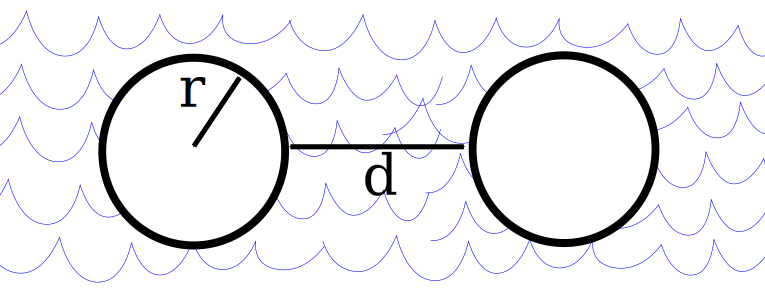
\includegraphics[width=\columnwidth]{figs/rods-diagram}
\end{center}
\caption{ Cross section schematic for two hydrophobic rods immersed in water.
The radius and separation are shown.}
\label{fig:rods}
\end{figure}

\begin{figure}
\begin{center}
\includegraphics[width=\columnwidth]{figs/density-rods-in-water}
\end{center}
\caption{ Density profiles illustrating the transition from vapor 
to liquid water between the rods. The radius is 0.5~nm, the top figure is 
at a separation of 0.2~nm and the
bottom is 0.6~nm. Figure~\ref{fig:rods-energy-vs-distance} shows
the energy for these and other separations.}
\label{fig:density-rods}
\end{figure}

The free energy per length is compared for rods of several different radii
in Figure~\ref{fig:rods-energy-vs-distance}. For ease of comparison, we 
arbitrarily offset each free energy such that they all go 
to zero at large separations. For large $d$, the rods 
simply act like two separate single rods in water and the energy will
reach an asymptote determined by the effective surface tension (shown in 
Figure~\ref{fig:energy-vs-diameter}). For small $d$, we see that all the rods 
have the same behavior, with a positive linear relationship
between free energy per length and separation during the initial state 
(where the rods have vapor between them). This indicates that the force 
per length on the rods is constant, and surprisingly independent of separation. 
By finding the slope of this curve, we calculate this force per length to be 144~mN/m.

\begin{figure}
\begin{center}
\includegraphics[width=\columnwidth]{figs/rods-energy-vs-distance}
\end{center}
\caption{ Free energy of hydration (also known as the potential of mean force) 
versus separation for two hydrophobic rods ranging in radius from
0.3~nm to 1.0~nm.
All were arbitrarily offset to zero at large separations. The
transition corresponds to the phase change from
vapor to liquid between the rods as pictured in the density profiles in 
Figure~\ref{fig:density-rods}. }
\label{fig:rods-energy-vs-distance}
\end{figure}

To explain this, we consider a macroscopic surface
tension model where the free energy in the macroscopic limit is given by 
\begin{equation}
F = \gamma A + pV
\end{equation}
The first term describes the surface energy and the second term
is the work needed to create a cavity of volume $V$. Since this pressure term
scales with volume, it can be neglected relative to the surface term provided
the length scale is small compared with $\frac{\gamma} p$. At room temperature,
the value of $\frac{\gamma} p$ is equal to about $20~\mu m$ which is
much larger than any of the solutes we study. We expect that for larger 
rods ... \needsworknow{Explain ``bowing'' out of vapor area for larger rods.}

Starting from the surface energy term, we can calculate the 
free energy per 
length, which is equal to the circumference multiplied by the surface tenson. 
The force
per length is the derivative of this with respect to the separation. 
We approximate the circumference of the stadium-shape by
\begin{equation}
C_{s} = 2\pi r +4r+2d
\end{equation}
and so the force per length is equal to $2\gamma$.

This is consistent with the calculation of the force per length from 
Figure~\ref{fig:rods-energy-vs-distance} (144~mN/m) and the surface tension 
in Figure~\ref{fig:surface-tension} (72~mN/m). This indicates that
even though the rods are nanoscale, the water molecules will ``see'' them classically.

To estimate how the transition from vapor to liquid between the rods depends on their 
radius, we will again use this model and propose that 
the critical separation, $d_c$, will occur when the free energies are equal. This 
corresponds to equating the circumference of the stadium-shape (see 
top of Figure~\ref{fig:density-rods}) and the circumference of the two rods (see bottom
of Figure~\ref{fig:density-rods}), which results in
\begin{equation}
d_c = (\pi-2)r.\label{criticalseparation}
\end{equation}
The predicted and actual computed values for $d_c$ are shown in 
Table~\ref{criticalseparationtable}, and they match fairly well for the 
0.5~-~1.0~nm rods. We hypothesize that larger radii rods
would also follow this trend, but smaller rods are likely to have a different
relationship with the surrounding water molecules. This may explain why the critical
separation result for a radius of 0.3~nm does not match the prediction well.

Walther \emph{et al.}\cite{walther2004hydrodynamic} studied the interactions between two
carbon nanotubes, which are geometrically similar to our hydrophobic rods. 
They use molecular dynamics with Lennard-Jones potentials for
nanotubes of diameter 1.25~nm and separations ranging from about 0.3~nm to 1.5~nm.
They also find that a drying transition occurs, and find it to be at separations near
0.9~-~1.0~nm\cite{walther2004hydrodynamic}. This is larger than
what we find for hydrophobic rods of a similar size, as expected due to the carbon-carbon
and carbon-water interations. 

\begin{table}
\begin{tabular} {|c|c|c|c|}
\hline
$r$ (nm) & $d_c$ prediction (nm) & $d_c$ result (nm) & \% error \\
\hline
0.3 & 0.34 & 0.23 & 32\% \\
\hline
0.5 & 0.57 & 0.54 & 5.3\% \\
\hline
0.7 & 0.80 & 0.81 & 1.3\% \\
\hline
0.9 & 1.03 & 1.06 & 2.9\% \\
\hline
1.0 & 1.14 & 1.19 & 4.4\% \\
\hline
\end{tabular}
\caption{Calculations of the critical separation 
(see Equation~\ref{criticalseparation})
for the transition
from liquid to vapor between two hydrophobic rods.\needsworknow{Delete
this table and move some of the information into the text along with
prediction model and explanation of Figure~\ref{fig:rods-energy-vs-distance}}.}
\label{criticalseparationtable}
\end{table} 

\subsection{Hydrophobic interactions of four rods}

%%%%%%%%%%%%%%%%%%%%%%%%%%%%%%%%%%%%%%%%%%%%%%%%%%%%%%%%%%%%
% 
% \subsection{Test-particle approach}
% 
% More interesting applications are possible when we move into three
% dimensions using spherical coordinates.  The first (but not simplest)
% thing to try is looking at the response of liquid water to a single
% fixed water molecule.  This is referred to as the \emph{test particle}
% method, and is as simple as constraining the density to
% include a delta function at the origin---meaning that a single
% molecule is fixed in location.  The free energy is then minimized
% under this constraint, giving a density profile and an associated free
% energy.  The density profile is just the self-correlation function
% multiplied by the bulk liquid density.  \fixme{We should be
%   distinguishing between the properties of the \emph{exact functional}
%   and those of an approximate functional...}  Thus, a test-particle
% calculation provides a stringent test of the correctness of any
% approximate functional.
% 
% In order to perform the test-particle test, we introduce a sharp
% gaussian density spike at the origin and relax the density under a
% constraint that this spike remain.  Figure~\ref{fig:test-particle}
% shows the resulting density profile, compared with the experimental
% $g_{\textrm{OO}}$.  Note that this data was \emph{not} used in the
% fitting of the empirical parameters of the functional.  The agreement
% between experiment and theory is both qualitatively and quantitatively
% poor.  The integral of the difference between this density profile
% (excluding the delta function) and the bulk liquid density should be
% 0.06~molecules \fixme{look up and show derivation... or cut this},
% but we find instead to be $-0.15$~molecules.  In addition, the associated
% free energy should be positive: there is an entropic cost in fixing
% one molecule in position, but for our functional the free energy of
% this density configuration is in fact negative, with a value of
% -3.5~eV, meaning that the homogeneous fluid is unstable.  This is a
% serious flaw that must be addressed in future work.
%
%%%%%%%%%%%%%%%%%%%%%%%%%%%%%%%%%%%%%%%%%%%%%%%%%%%%%%%

\subsection{Hydration energy of hard-sphere solutes}

\begin{figure}
\begin{center}
\includegraphics[width=\columnwidth]{figs/sphere-energy-vs-diameter}
\end{center}
\caption{ Free energy versus radius for a single hydrophobic sphere
  immersed in water. This should have an asymptote equal to the
  surface tension at room temperature, and it agrees well with the
  surface tension in Figure~\ref{fig:surface-tension}. Results from a
  simulation of SPC/E water~\cite{huang2001shs} are shown as circles.
  The horizonal lines show the experimental and SPC/E bulk surface
  tension for water at standard atmospheric temperature and
  pressure. }
\label{fig:sphere-energy-vs-diameter}
\end{figure}

A common model of hydrophobic solutes is the \emph{hard sphere solute}
\fixme{add citations?}.  The effect of this solute is merely to create
a cavity within which the water may not penetrate.  This is the
simples possible solute, and will serve as a test case, which if
passed could lead to the ability to insert different chemicals into
aqueous solution, instead of a vapor cavity, in order to observe
biologically and chemically important aqueous solvation interactions.

As in the single rod, we begin by examining the free energy of
hydration, expressed in Figure~\ref{fig:sphere-energy-vs-diameter} as
the ratio of the energy of the cavity system to the surface area of
the cavity.  This \emph{effective surface tension}, approaches the
bulk surface tension as the cavity radius increases.  As with the
single rod, we see the analytically correct behavior in the limit of
small solutes.  We also plot the surface tension calculated using a
molecular dynamics simulation of SPC/E water\cite{huang2001shs}.  The
agreement is quite excellent, apart from the issue that the SPC/E
model for water significantly underestimates the surface tension of
water at room temperature\cite{vega2007surface}.

Figure~\ref{fig:density-sphere} shows the density profile for several
hard sphere radii, plotted together with with the results of the same
SPC/E molecular dynamics simulation shown in
Figure~\ref{fig:sphere-energy-vs-diameter}\cite{huang2001shs}.  The
agreement with simulation is quite reasonable.  The largest
disagreement involves the density at contact, which according to the
contact value theorem cannot agree, since the free energies do not
agree.

\begin{figure}
\begin{center}
\includegraphics[width=\columnwidth]{figs/sphere-density}
\end{center}
\caption{ Density profiles illustrating the transition from vapor 
to liquid water between the rods. The radius is 0.5~nm, the top figure is 
at a separation of 0.2~nm and the
bottom is 0.6~nm. Figures~\ref{fig:rods-energy-vs-distance}~and~\ref{fig:energy-rods} show
the energy for these and other separations.}
\label{fig:sphere-density}
\end{figure}


\begin{figure}
\begin{center}
\includegraphics[width=\columnwidth]{figs/density-sphere}
\end{center}
\caption{ Density profiles around hard-sphere solutes of different radii. Predictions
  from our classical density-functional theory are in solid red, while
  the dotted line shows the result of a molecular dynamics simulation
  of SPC/E water~\cite{huang2001shs}.  }
\label{fig:density-sphere}
\end{figure}

\section{Conclusion}

The classical density functional we developed by combining fundamental-measure 
theory with SAFT is able to produce reasonable results for hydrophobic interations.
We added the parameter $\lscale$ to the functional and fit it to the surface tension
at room temperature, which we find to be consistent with results for larger hydrophobic
rods. 

The free energy per area for water surrounding a hydrophobic rod shows the
expected behavior with an asymptote equal to the surface tension.
Based on this result, we expect to be
able to classically describe rods with a radius of about 0.5~nm or larger. 
For two hydrophobic rods surrounded by water, we see a transition from a vapor-filled
stadium shape to two rods with liquid between them. A
classical treatment of the critical separation for this transition
works well for rods larger than 0.5~nm. Further evidence for the
accuracy of this classical treatment is the calculation of the force on the
stadium shape. The force per length is constant and equal to twice the surface tension.

For the hydrophobic systems studied, this functional is more computationally 
efficient than molecular dynamics. This allows for future work
involving hydrophilic interactions with more complex electrostatic interactions.


\bibliography{paper}% Produces the bibliography via BibTeX.

\end{document}

